% ============================================
% 4 问题1：风化规律与风化前成分预测
% ============================================
\section{问题1：风化规律与风化前成分预测}

\subsection{风化与类型、纹饰、颜色的关联分析}

\subsubsection{数据预处理}

从表单1读取 58 件文物基本信息。颜色字段存在 4 件缺失（编号 19、40、48、58），对低频颜色（出现次数 $< 5$）合并为"其他"类别以保证列联表检验的有效性。

\subsubsection{研究方法}

构建各因素与风化状态的 $2 \times 2$（类型）或 $3 \times 2$（纹饰、颜色）列联表：
\begin{itemize}
    \item \textbf{类型 $\times$ 风化}：$2 \times 2$ 列联表，采用 Fisher 精确检验（小样本适用）
    \item \textbf{纹饰 $\times$ 风化}：$3 \times 2$ 列联表，采用卡方检验，计算 Cramér's $V$ 效应量
    \item \textbf{颜色 $\times$ 风化}：列联表，卡方检验
\end{itemize}

显著性水平 $\alpha = 0.05$，三次同时检验采用 Bonferroni 校正（$\alpha' = 0.0167$）。

\subsubsection{结果分析}

\begin{table}[H]
    \centering
    \caption{风化关联分析检验结果}
    \label{tab:weathering_test}
    \begin{tabular}{l c c c c}
        \toprule
        \textbf{因素} & \textbf{检验方法} & \textbf{$p$ 值} & \textbf{效应量} & \textbf{结论} \\
        \midrule
        玻璃类型 & Fisher Exact & \textbf{0.0113} & —— & 显著 \\
        纹饰 & Chi-square & 0.0839 & $V = 0.292$ & 不显著 \\
        颜色 & Chi-square & 0.9951 & $V = 0.035$ & 不显著 \\
        \bottomrule
    \end{tabular}
\end{table}

\begin{itemize}
    \item 高钾玻璃风化率：$33.3\%$（6/18）
    \item 铅钡玻璃风化率：$70.0\%$（28/40）
\end{itemize}

\textbf{结论}：玻璃类型是影响风化的唯一显著因素。铅钡玻璃因化学稳定性较差，风化率远高于高钾玻璃。纹饰 B 类 $100\%$ 风化率可能受样本量小（$n=6$）影响。颜色与风化无关（$p=0.995$），颜色主要受着色剂（CuO、$\text{Fe}_2\text{O}_3$）影响，与风化机制无直接关联。

\begin{figure}[H]
    \centering
    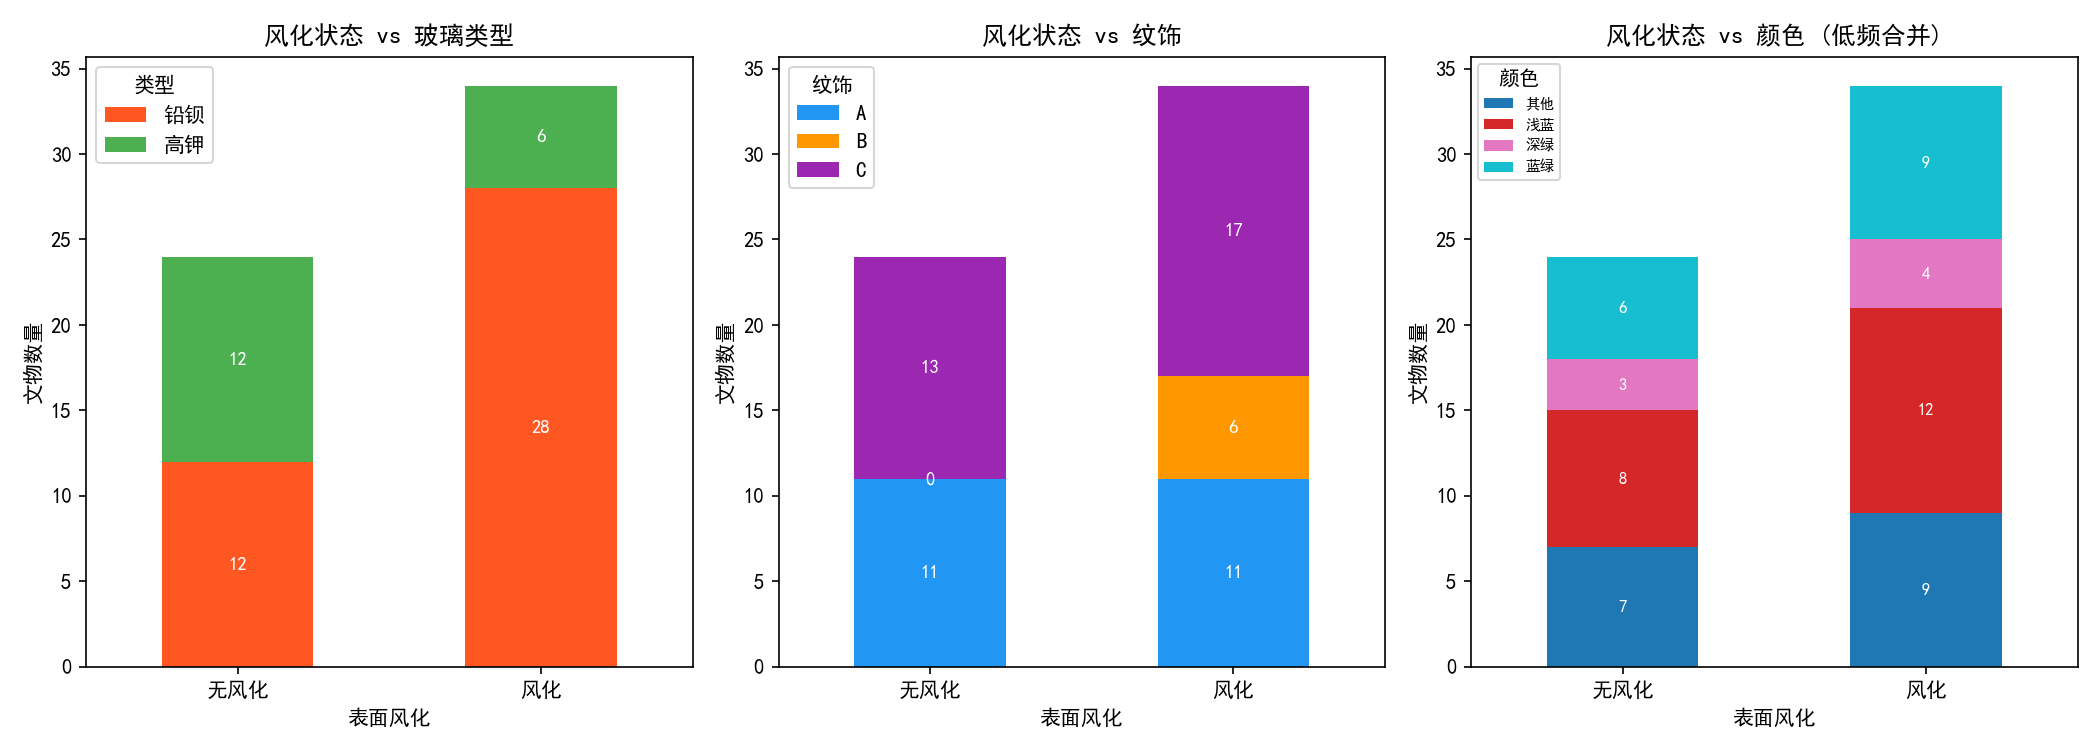
\includegraphics[width=0.85\textwidth]{../analysis/fig1a_weathering_relations.png}
    \caption{风化关联分析堆叠柱状图（左：风化$\times$类型；中：风化$\times$纹饰；右：风化$\times$颜色）}
    \label{fig:weathering_relation}
\end{figure}

\subsection{风化前后化学成分统计规律}

\subsubsection{数据准备}

合并表单1与表单2，得到 69 条采样数据，排除 2 条总和不在 $85\%\sim105\%$ 范围内的无效数据，保留 67 条。按 [类型 $\times$ 风化状态] 分为 4 组：

\begin{table}[H]
    \centering
    \caption{四组数据划分}
    \label{tab:four_groups}
    \begin{tabular}{l c}
        \toprule
        \textbf{组别} & \textbf{样本量} \\
        \midrule
        高钾-无风化 & 12 \\
        高钾-风化 & 6 \\
        铅钡-无风化 & 13 \\
        铅钡-风化 & 36 \\
        \bottomrule
    \end{tabular}
\end{table}

\subsubsection{研究方法}

对每种氧化物进行分组统计（均值 $\pm$ 标准差），计算风化差异 $\Delta =$ 风化组均值 $-$ 无风化组均值。采用 Mann-Whitney U 检验（非参数方法，适用于小样本和非正态分布）评估风化效应的统计显著性，并进行 Bonferroni 多重检验校正。配对验证：利用文物 08、26、54 的"严重风化点"与同文物普通采样点进行配对比较。

\subsubsection{结果分析}

\textbf{高钾玻璃风化效应}：

\begin{table}[H]
    \centering
    \caption{高钾玻璃风化前后主要氧化物变化}
    \label{tab:hk_weathering}
    \begin{tabular}{l c c c c}
        \toprule
        \textbf{氧化物} & \textbf{未风化均值} & \textbf{风化均值} & \textbf{变化量 $\Delta$} & \textbf{相对变化} \\
        \midrule
        $\text{SiO}_2$ & 68.0\% & 94.0\% & \textbf{$+26.0\%$} & $+38.2\%$ \\
        $\text{K}_2\text{O}$ & 9.3\% & 0.5\% & \textbf{$-8.8\%$} & $-94.2\%$ \\
        $\text{Al}_2\text{O}_3$ & 6.6\% & 1.9\% & $-4.7\%$ & $-70.8\%$ \\
        CaO & 5.3\% & 0.9\% & $-4.5\%$ & $-83.7\%$ \\
        \bottomrule
    \end{tabular}
\end{table}

风化后高钾玻璃几乎只剩 $\text{SiO}_2$——$\text{K}_2\text{O}$、$\text{Na}_2\text{O}$、CaO、MgO 等可溶成分全部流失。$\text{SiO}_2$ 的升高是相对富集效应（其他成分流失导致 $\text{SiO}_2$ 占比被动上升），而非 $\text{SiO}_2$ 绝对含量增加。

\textbf{铅钡玻璃风化效应}：

\begin{table}[H]
    \centering
    \caption{铅钡玻璃风化前后主要氧化物变化}
    \label{tab:pb_weathering}
    \begin{tabular}{l c c c c}
        \toprule
        \textbf{氧化物} & \textbf{未风化均值} & \textbf{风化均值} & \textbf{变化量 $\Delta$} & \textbf{相对变化} \\
        \midrule
        $\text{SiO}_2$ & 53.4\% & 33.6\% & \textbf{$-19.8\%$} & $-37.1\%$ \\
        PbO & 23.6\% & 36.9\% & \textbf{$+13.3\%$} & $+56.3\%$ \\
        $\text{P}_2\text{O}_5$ & 0.9\% & 4.2\% & $+3.3\%$ & $+359.7\%$ \\
        $\text{SO}_2$ & 0.3\% & 1.0\% & $+0.7\%$ & $+250.5\%$ \\
        \bottomrule
    \end{tabular}
\end{table}

PbO 相对富集（不易流失的重元素），$\text{P}_2\text{O}_5$/$\text{SO}_2$ 大幅增加（环境元素进入）。配对验证（08、26、54 严重风化点 vs 普通点）一致显示 $\text{SiO}_2$ 降低、$\text{SO}_2$ 和 $\text{P}_2\text{O}_5$ 升高，证实风化为 $\text{SiO}_2$ 流失 $+$ 环境元素进入的双向交换过程。

\textbf{统计显著性}（Bonferroni 校正后）：
\begin{itemize}
    \item 高钾：$\text{SiO}_2$（$p = 0.003$）和 $\text{Al}_2\text{O}_3$（$p = 0.006$）变化显著
    \item 铅钡：仅 $\text{SiO}_2$（$p = 0.020$）变化显著
\end{itemize}

\begin{figure}[H]
    \centering
    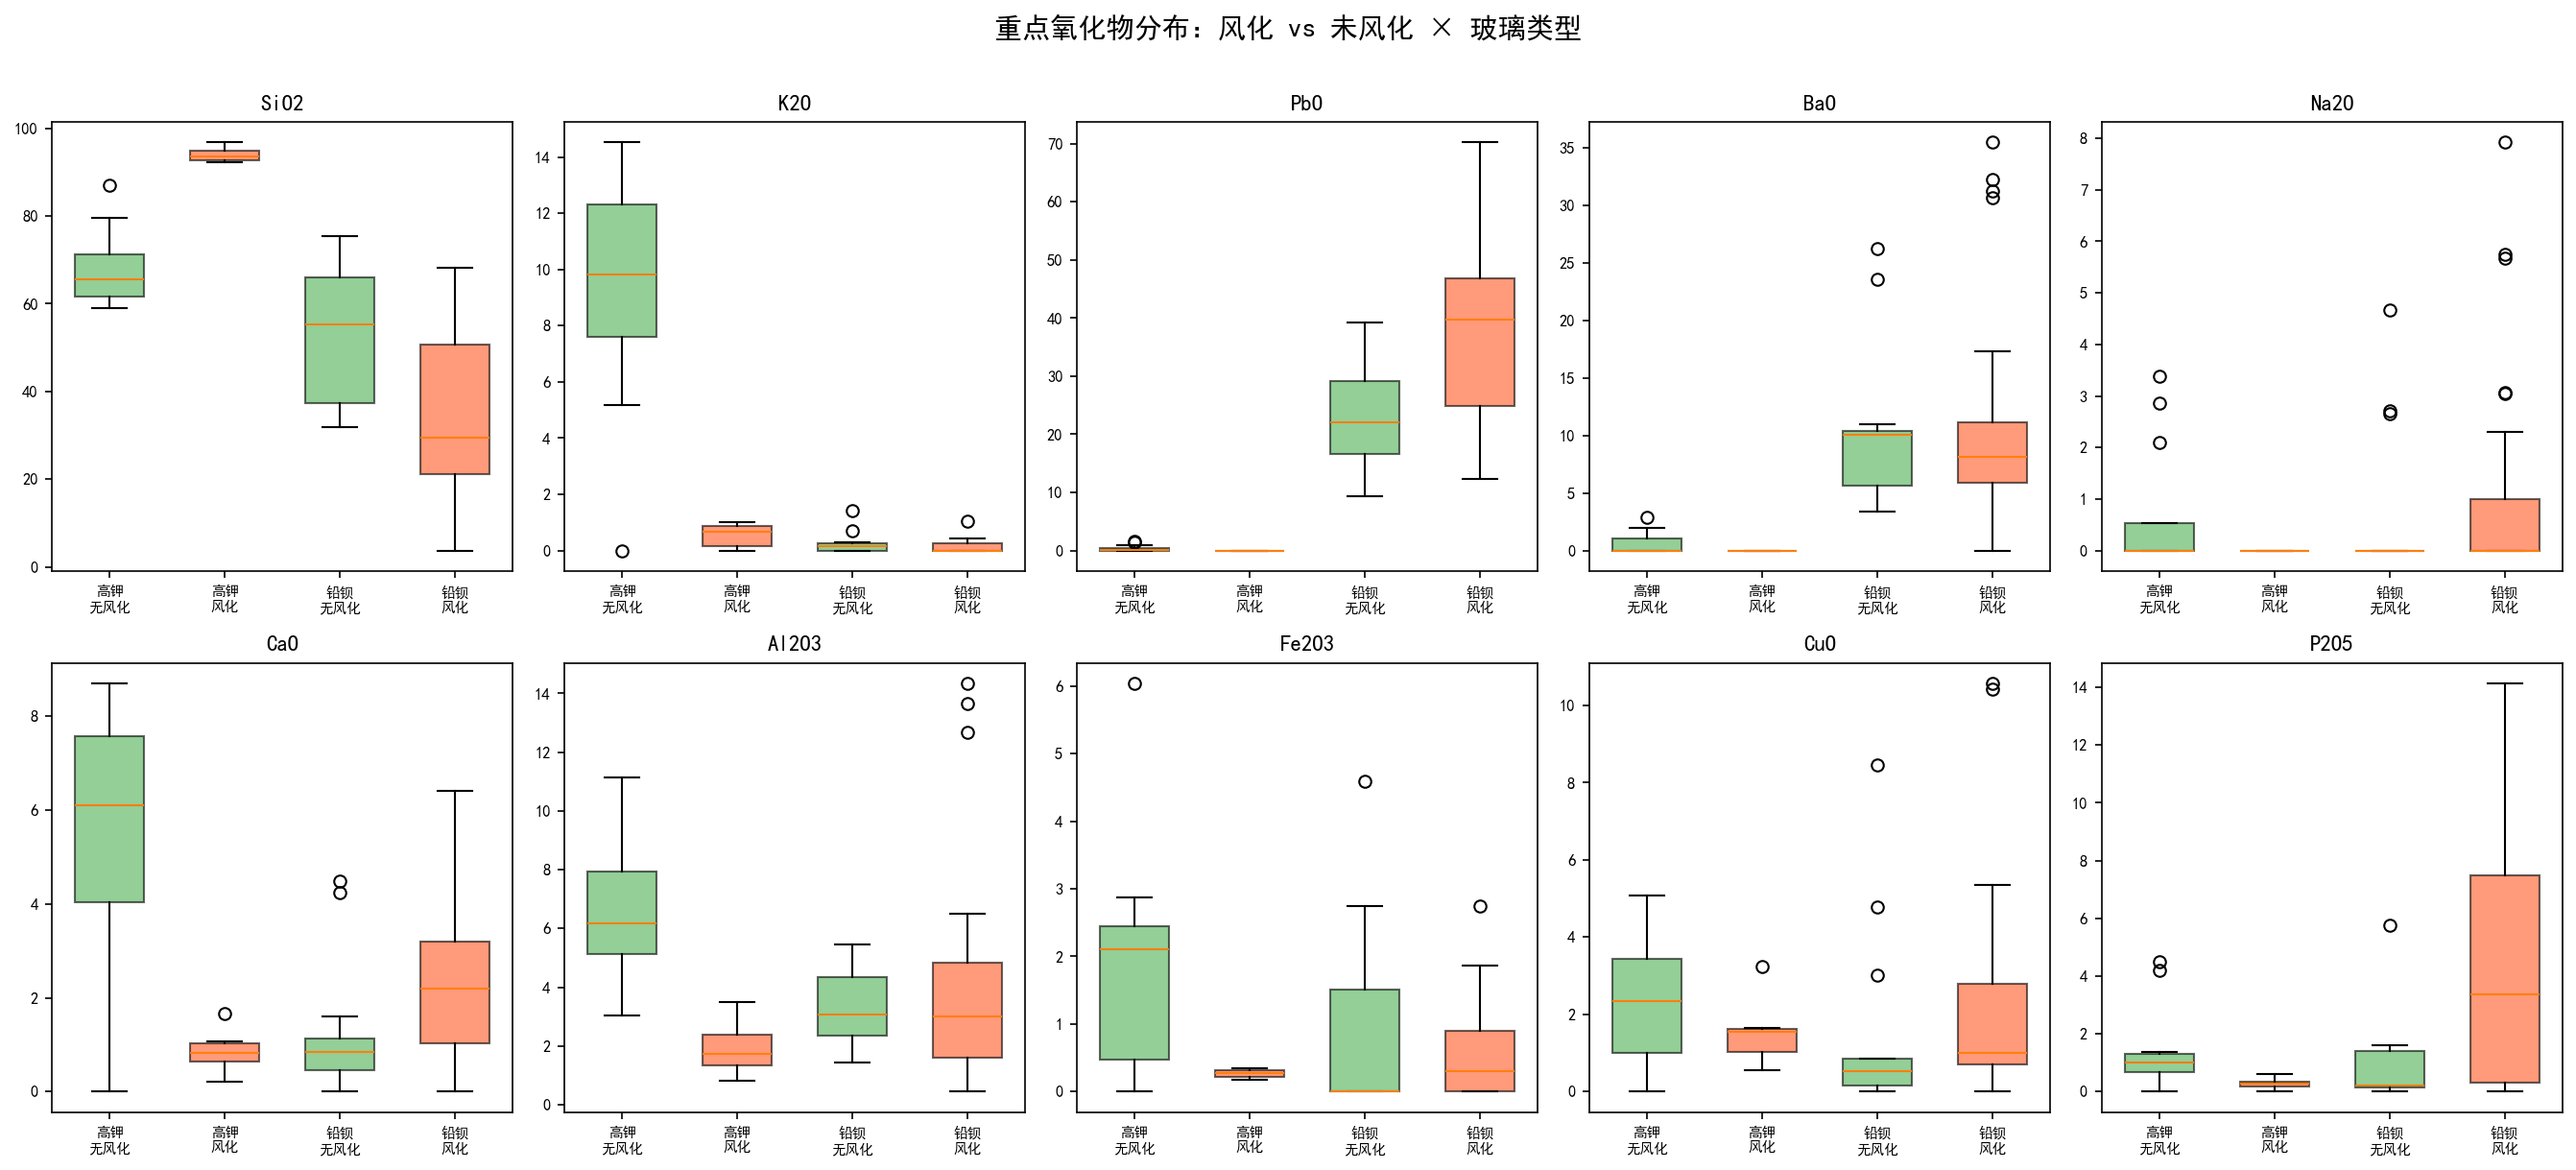
\includegraphics[width=0.85\textwidth]{../analysis/fig1b_boxplots.png}
    \caption{风化前后化学成分箱线图}
    \label{fig:boxplots}
\end{figure}

\begin{figure}[H]
    \centering
    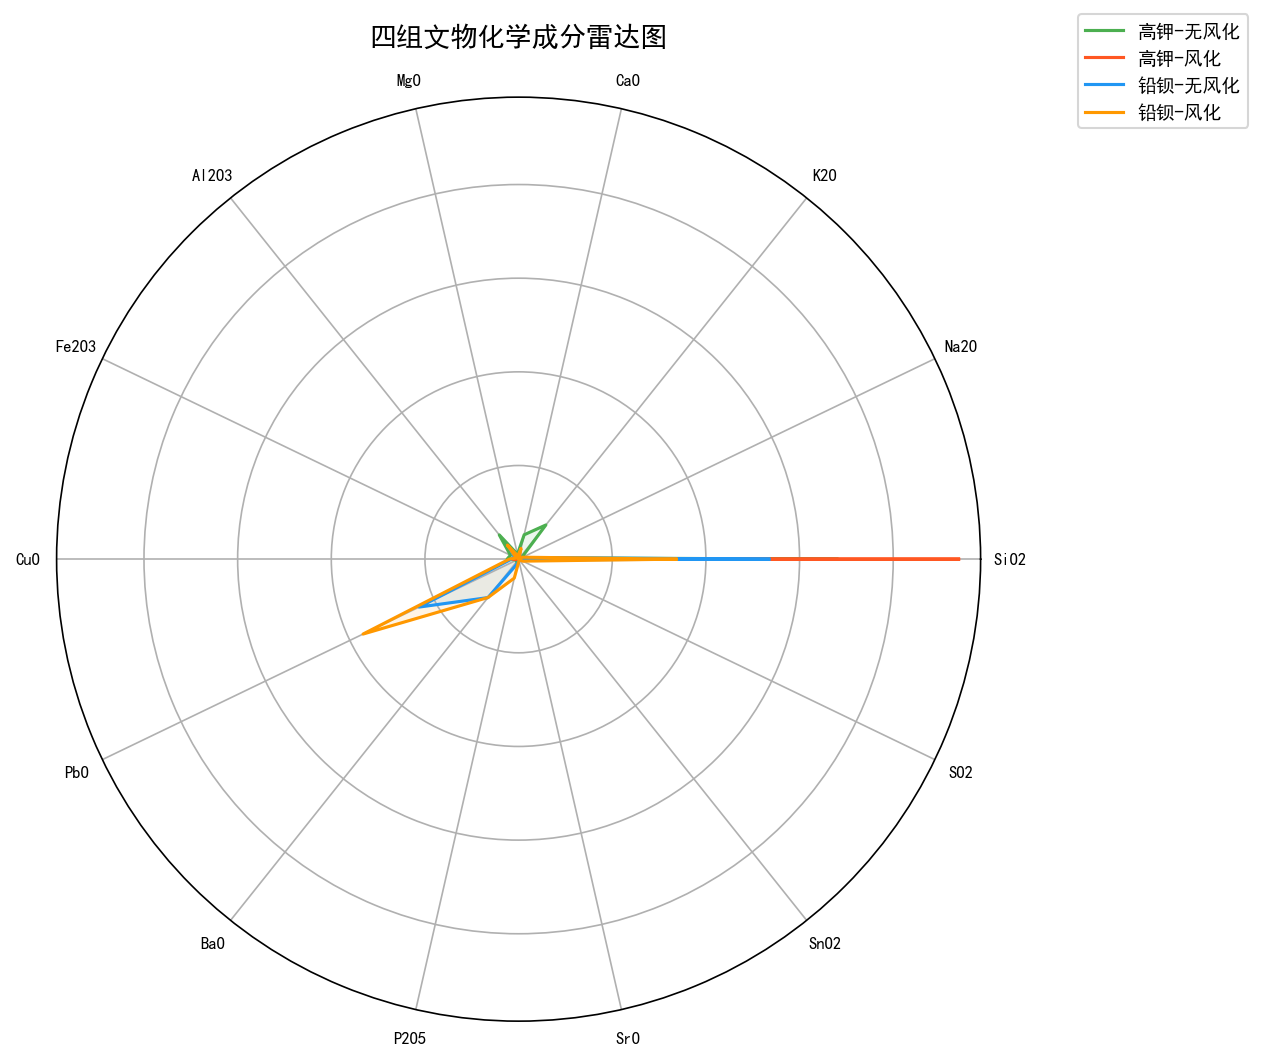
\includegraphics[width=0.8\textwidth]{../analysis/fig1b_radar.png}
    \caption{四组化学成分雷达图}
    \label{fig:radar}
\end{figure}

\begin{figure}[H]
    \centering
    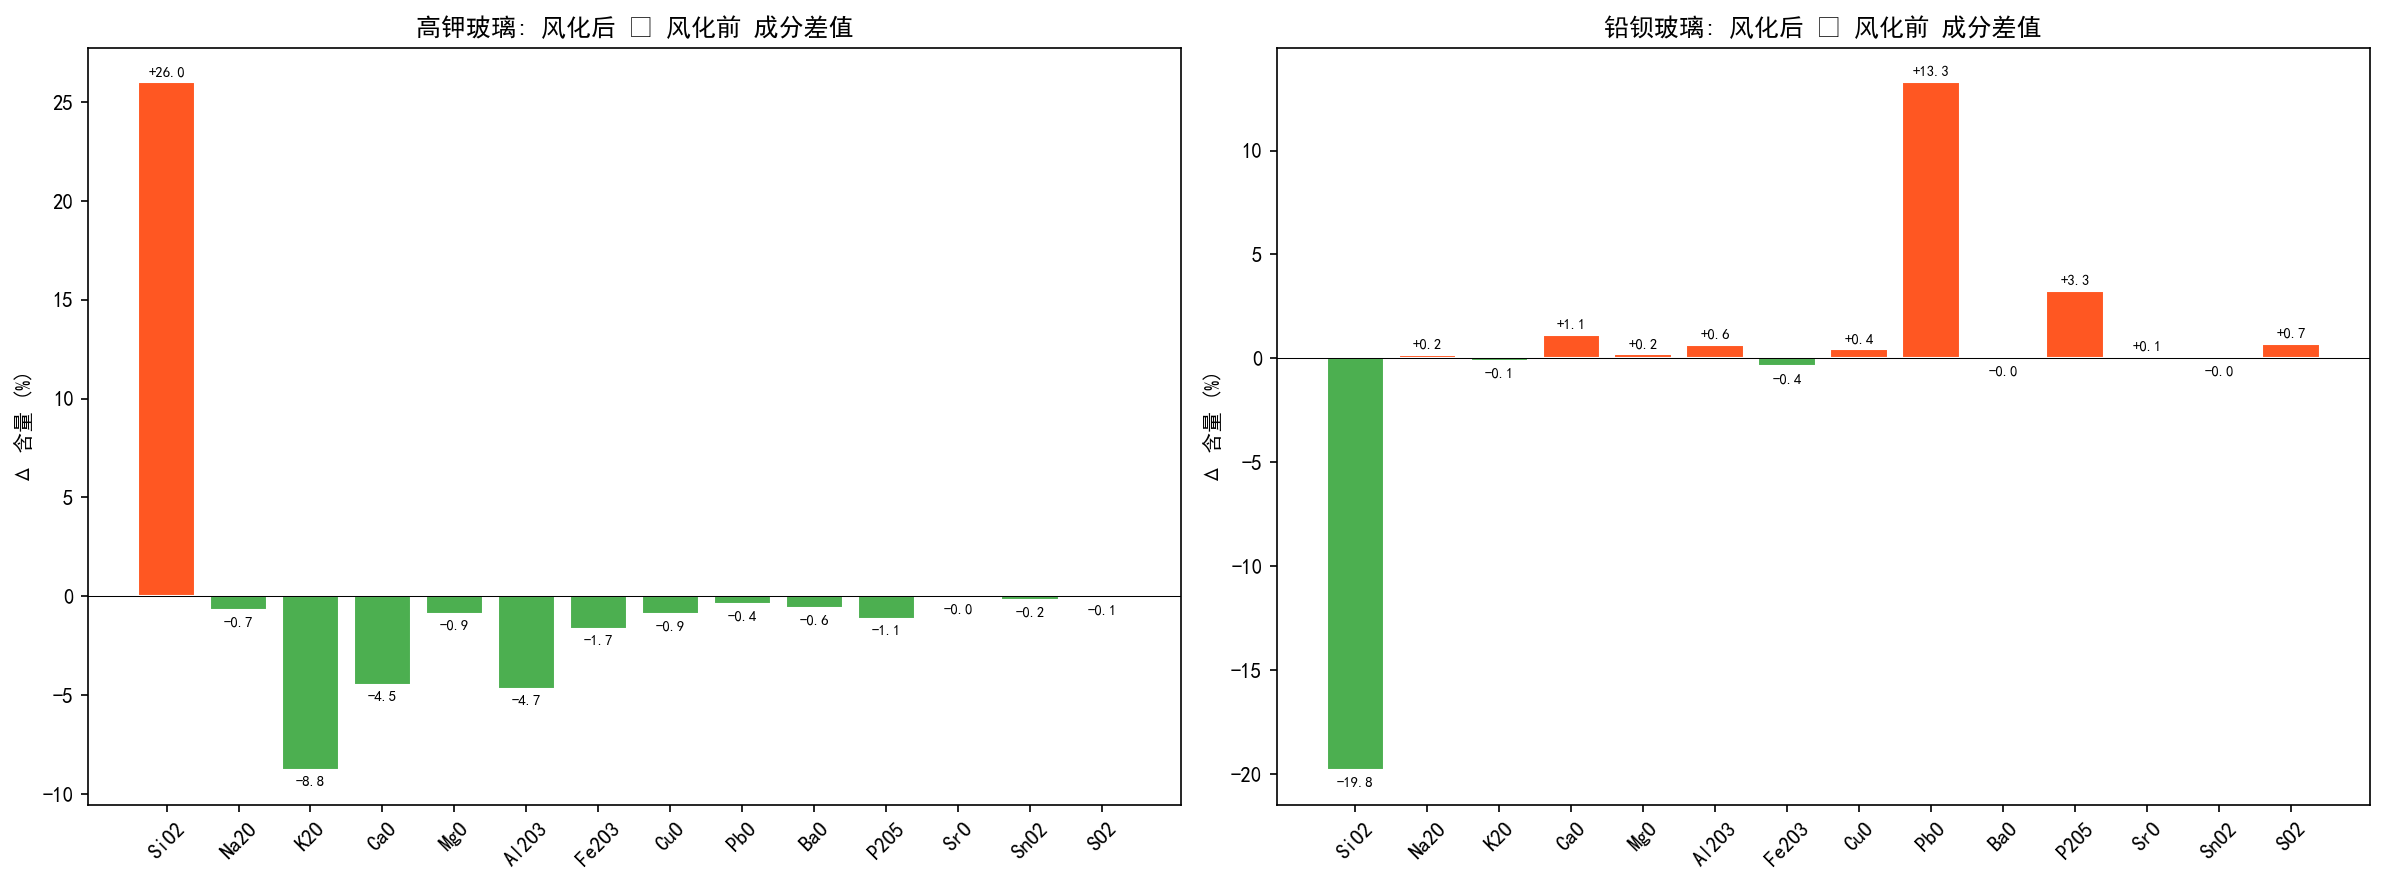
\includegraphics[width=0.8\textwidth]{../analysis/fig1b_diff_bar.png}
    \caption{风化效应差值棒图（高钾 vs 铅钡）}
    \label{fig:diff_bar}
\end{figure}

\subsection{风化前化学成分预测}

\subsubsection{研究方法}

建立\textbf{分类型差值校正模型}：

\begin{equation}
    C_{ij}^{\text{pre}} = C_{ij}^{\text{post}} - \Delta_j
\end{equation}

其中 $\Delta_j$ 为第 $j$ 种氧化物的风化效应向量，按类型分别计算：

\begin{itemize}
    \item \textbf{铅钡玻璃}：利用文物 49、50 的配对样本（未风化点 vs 普通采样点），$\Delta =$ 风化后 $-$ 风化前均值。共 2 对配对样本。
    \item \textbf{高钾玻璃}：利用组间均值差，$\Delta =$ 风化组均值（$n = 6$）$-$ 无风化组均值（$n = 12$）。
\end{itemize}

校正后结果 clip 到 $[0, 100]$ 区间。

\subsubsection{校正向量}

\textbf{高钾玻璃校正向量}（正值 $=$ 风化后增加，需减去）：
\begin{itemize}
    \item $\text{SiO}_2$: $+26.0\%$、$\text{K}_2\text{O}$: $-8.8\%$、$\text{Al}_2\text{O}_3$: $-4.7\%$、CaO: $-4.5\%$
    \item 其余微量元素全部流失至接近 $0\%$
\end{itemize}

\textbf{铅钡玻璃校正向量}：
\begin{itemize}
    \item $\text{SiO}_2$: $-19.8\%$、PbO: $+13.3\%$、$\text{P}_2\text{O}_5$: $+3.3\%$、BaO: $-0.01\%$、$\text{SO}_2$: $+0.7\%$
\end{itemize}

\subsubsection{模型验证}

留出验证（文物 49、50，预测其未风化点成分并与实测值比较）：

\begin{table}[H]
    \centering
    \caption{风化前成分预测验证结果}
    \label{tab:predict_validation}
    \begin{tabular}{l c c c}
        \toprule
        \textbf{文物} & \textbf{MAE} & \textbf{$\text{SiO}_2$ 误差} & \textbf{PbO 误差} \\
        \midrule
        49 & 0.79\% & $+0.61\%$ & $-1.11\%$ \\
        50 & 0.75\% & $-0.61\%$ & $+1.12\%$ \\
        \bottomrule
    \end{tabular}
\end{table}

关键氧化物（$\text{SiO}_2$、PbO）预测误差 $< 1.5\%$，模型精度良好。BaO 和 $\text{P}_2\text{O}_5$ 误差较大（$3\%\sim4\%$），因这两者在风化交换中最为活跃、个体差异大。

\subsubsection{局限性}

\begin{enumerate}[label=(\arabic*)]
    \item 铅钡校正仅基于 2 对样本，统计代表性有限
    \item 高钾校正基于组间均值，未考虑文物间个体差异
    \item 环境元素（$\text{SO}_2$、$\text{P}_2\text{O}_5$）的风化交换过程非线性，简单差值法无法完全捕捉
\end{enumerate}

\begin{figure}[H]
    \centering
    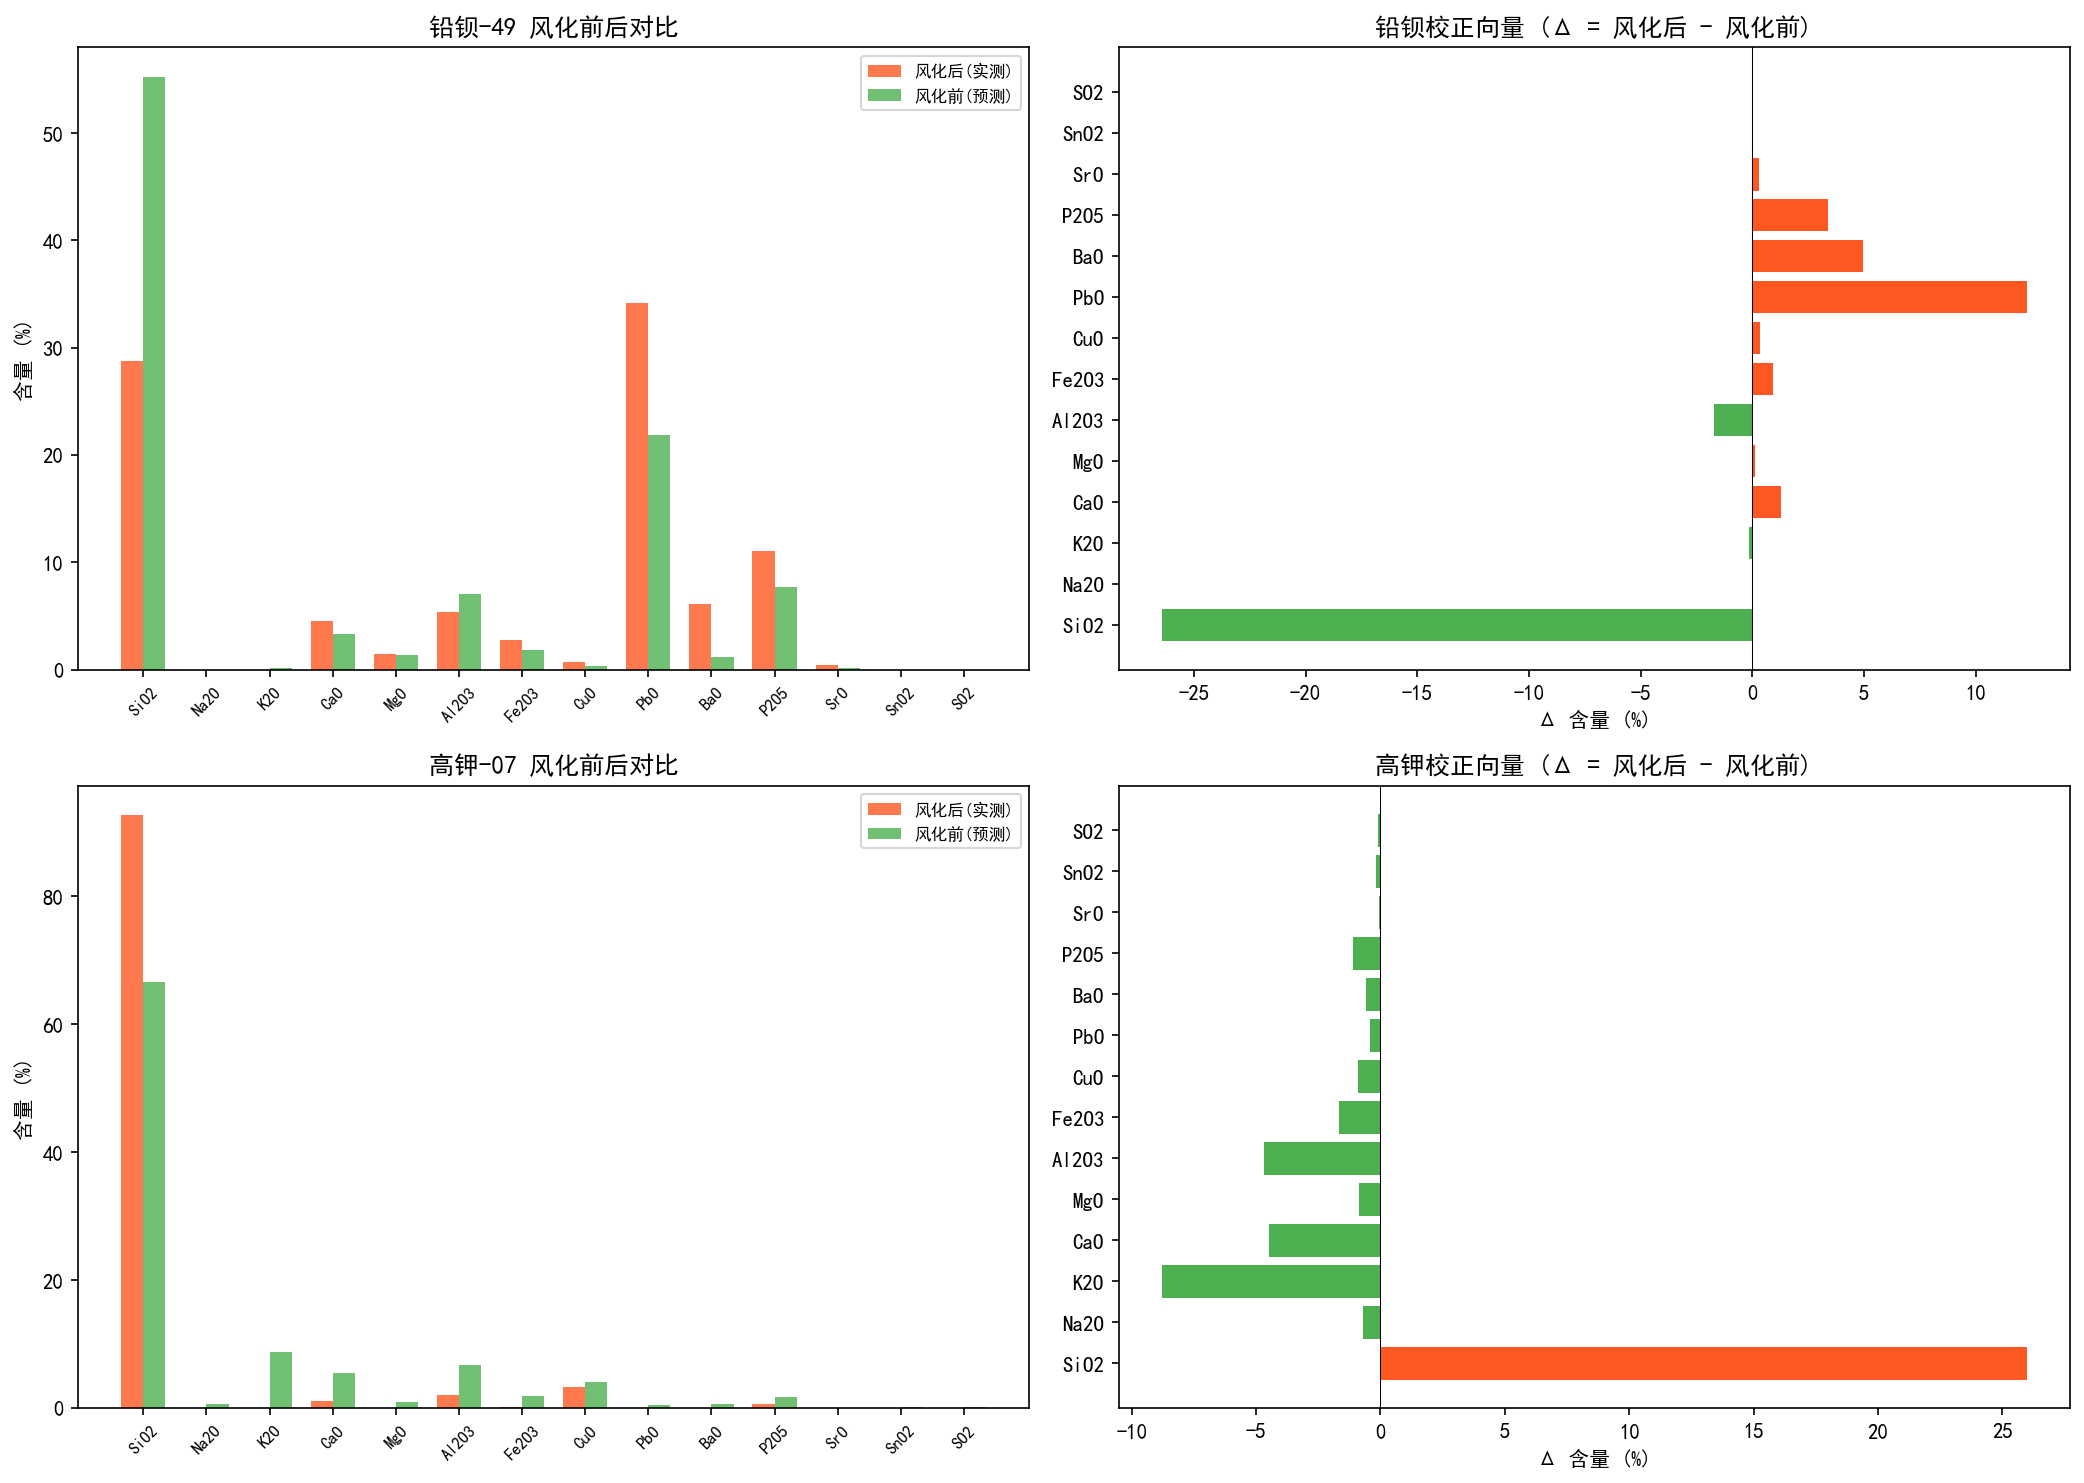
\includegraphics[width=0.85\textwidth]{../analysis/fig1c_predictions.png}
    \caption{风化前成分预测对比图（配对验证 + 校正向量）}
    \label{fig:predictions}
\end{figure}
